\documentclass{beamer}
%
% Choose how your presentation looks.
%
% For more themes, color themes and font themes, see:
% http://deic.uab.es/~iblanes/beamer_gallery/index_by_theme.html
%
\mode<presentation>
{
  \usetheme{Berlin}      % or try Darmstadt, Madrid, Warsaw, ...
  \usecolortheme{beaver} % or try albatross, beaver, crane, ...
  \usefonttheme{default}  % or try serif, structurebold, ...
  \setbeamertemplate{navigation symbols}{}
  \setbeamertemplate{caption}[numbered]
} 

\usepackage[english]{babel}
\usepackage[utf8x]{inputenc}
\usepackage{tikz}
\usepackage{amsmath}
\usepackage{verbatim}
\usetikzlibrary{arrows,shapes}
\usepackage{xcolor}
\usepackage{hyperref}
 
\newcommand{\highlight}[1]{%
  \colorbox{red!50}{$\displaystyle#1$}}
\setcounter{tocdepth}{1}

\title[j-logic]{Proof Search for Justification Logic in Python}
\author{Judith Fuog}
\institute{Universität Bern, Informatik}
\date{13. Nov 2014}

\begin{document}

\begin{frame}
  \titlepage
\end{frame}

% Uncomment these lines for an automatically generated outline.
\begin{frame}{Outline}
  \tableofcontents
\end{frame}

\section{Introduction}
\subsection{Motivation}
\begin{frame}{Motivation}
	Combination of
	\begin{itemize}
		\item practical coding in a modern language
		\item contribute to something existing
		\item riddling around with logic
	\end{itemize}
\end{frame}

\subsection{Requirements}
\begin{frame}{Early Stage}
	Extend an existing project to also handle Justification Logic.
	\begin{description}
	\item[Z3]Theorem prover from Microsoft Research. It can be used to check the satisfiability of logical formulas over one or more theories.\\
	\url{http://z3.codeplex.com/}
	\end{description}
	Available APIs
	\begin{itemize}
	\item Python
	\item C, C++, .NET, Java
	\end{itemize}
\end{frame}

\begin{frame}{Later}
	Implement a stand-alone algorithm for proof search in Justification Logic.

	Input:		
		\begin{itemize}
			\item Correct formatted String of a formula with a \emph{constant specification} list.
			\item Formula may only contain Justification Logic operations and implication ($\to$).
		\end{itemize}
		
	Output:
		\begin{itemize}
			\item If formula is provable.\\
			(True or False)
		\end{itemize}
	No time restriction or special care for efficiency.
\end{frame}

\subsection{Technologies and Methods}
\begin{frame}{Technologies}
	\begin{itemize}	
	\item[Python] Although the idea of extending \emph{Z3} was dropped the choice of the language remained.	
	\begin{itemize}
		\item version 3.x
		\item unit tests: module \texttt{unittest}
	\end{itemize}
		\item[pyCharm] IDE for Python
		\item[git] for versioning
	\end{itemize}
	\end{frame}

\begin{frame}{Methods}
	\begin{itemize}
		\item[KISS] Simplify as much as possibly and make it run. Add more functionality later on.
		\item[Tests] Lots of tests
		\begin{itemize}
			\item Tests in advance (TDD)
			\item Tests for doubts
			\item Tests while debugging
		\end{itemize}
	\end{itemize}
\end{frame}

\subsection{Result}
\begin{frame}{Result}
	Basic requirement fulfilled including one addition.	
	\vspace{1cm}
	
	Code
	\begin{itemize}
		\item 4 classes, thereof \texttt{Tree} and \texttt{ProofSearch} most important.
		\item Test for all 4 classes. Number of tests vary greatly depending on the complexity of the function.
	\end{itemize}	
\end{frame}

\section{Structure}
\subsection{Justification Logic}
\begin{frame}{What is Justification Logic?}
	 Justifications logic are epistemic model logic that use a formal construct to formalize the justification of knowledge of a statement.
	\begin{block}{Formula \textbf{t:F}}
	\begin{itemize}
		\item[$t$] proof term $t$ is a justification for \textit{F}.
		\item[$F$] Axiom $F$ must satisfies conditions \textit{t}.
	\end{itemize}
	\end{block}	
\end{frame}

\begin{frame}{Basics of Justification Logic}
	\begin{block}{Rules for proof terms}
	\begin{itemize}
	\item[C1]$t:(F \to G), s:F \vdash t*s:G$
	\item[C2]$t:F \vdash (t+s):F$, $s:F \vdash (t+s):F$
	\item[C3]$t:F \vdash !t:t:F$
	\end{itemize}
	\end{block}
	\begin{block}{constant specification \textbf{CS}}
	Finite set of formulas of the form $(c:A)$ where $c$ is a proof constant and $A$ is one of the axioms \textbf{A0-A4}.
	\end{block}
\end{frame}

\begin{frame}{Example}
		Find if the following formula is provable for $CS$:
		\begin{itemize}
		\item $s:G$
		\item $((s*t)+(!s)):F$
		\item $...$
		\end{itemize}
		
		\begin{equation}
		CS = \{(s, (t:F)), (s, (G \to F)), \highlight{(s, G)}, (t, (s:G)), (t, G)\}		
		\end{equation}

		If the proof term is not constant, it must be broken down in pieces.
\end{frame}

\subsection{Data Structure}
\begin{frame}{Binary Tree}
	\begin{block}{Find order of operations}
	
	\begin{itemize}
	\item Regular Expressions? 
	\item Binary Trees!
	\end{itemize}
	\end{block}
	
	\tikzset{
  treenode/.style = {align=center, inner sep=0pt, text centered,
    font=\sffamily},
  arn_n/.style = {treenode, circle, white, font=\sffamily\bfseries, draw=black,
    fill=black, text width=1.5em},% arbre rouge noir, noeud noir
  arn_r/.style = {treenode, circle, red, draw=red, 
    text width=1.5em, very thick},% arbre rouge noir, noeud rouge
  arn_w/.style = {treenode, circle, draw=black, 
    text width=1.5em, very thick},% arbre rouge noir, noeud rouge
  arn_x/.style = {treenode, rectangle, draw=black,
    minimum width=0.5em, minimum height=0.5em}% arbre rouge noir, nil
	}
	\begin{center}	
	\begin{tikzpicture}[level distance=1cm,
	  level 1/.style={sibling distance=3cm},
	  level 2/.style={sibling distance=1.2cm}]
  	\node [arn_n]{:}
  	  child {node [arn_w]{\(+ \)}
  	    child {node [arn_w] {*}
  	    	child {node [arn_w] {s}}
  	    	child {node [arn_w] {t}}
  	    	}
  	    child {node [arn_w] {!}
  	    	child[right] {node [arn_w] {s}}
  	    	}
  	  }
  	  child {node [arn_w]{F}
    };
	\end{tikzpicture}
	\end{center}
\end{frame}


\subsubsection{Binary Trees}
\begin{frame}{Types}
	Often the data types are mixed such that it becomes very difficult to keep an overview.
	\begin{description}
		\item[String] Formulas are always passed as String, even if they change their type in between.
		\item[Dictionary] Pythons implementation of a Hash. 
		\item[Tuple] are immutable in Python. Used for conditions.
		\item[List] are used to represent tables among other uses. 
	\end{description}
	
	Example:\\
	\texttt{$[(\{'X1':'', 'X2':'C', 'X3':'B'\}, [('X2', 'X1'),... ]), ... ]$}
\end{frame}

\section{Algorithm}
\subsection{Strategy}
\begin{frame}{The Divide and Conquer Principle}
	\begin{block}{Problem}
	Straight-forward approach proved to hold to many cases to handle them all at once.
	\end{block}
	\begin{itemize}
	\item[divide]Take a formula apart till only the smallest parts remains.
		\begin{itemize} 
		\item atomize (sumspilt, simplify bang, remove bad bang) 
		\item get musts
		\end{itemize}
	\item[conquer]For each of these \textit{atoms} check if they are resolvable in CS.
		\begin{itemize}
		\item configurations and conditions
		\item merge
		\end{itemize}
	\end{itemize}	 
\end{frame}

\subsection{Divide}
\subsubsection{Atomize}
\begin{frame}{Atomize - Sumsplit}
	\begin{block}{}
	\begin{itemize}
		\item[C2]$t:F \vdash (t+s):F$, $s:F \vdash (t+s):F$
	\end{itemize}
	To check if provable for
	\[((s*t)+(!s)):F\]
	it is enough if (any) one of the parts is provable.
	\[(s*t):F, (!s):F\]
	\end{block}	
\end{frame}

\begin{frame}{Atomize - Simplify Bang}
	\begin{block}{}
	\begin{itemize}
		\item[C3]$t:F \vdash !t:(t:F)$
	\end{itemize}
	If a bang is first operation of the left subtree the left child of the right subtree must be the same as what is beneath the bang from the left subtree. So it is enough to simple check the right subtree.
		\[(!s):(s:G) \Rightarrow s:G\]
		\[(!s):F\ \Rightarrow \bot\]
	\end{block}
\end{frame}

\begin{frame}{Remove Bad Bang}
	\begin{block}{}
	\begin{itemize}
		\item[C1]$t:(F \to G), s:F \vdash t*s:G$
		\item[C3]$t:F \vdash !t:(t:F)$
	\end{itemize}
	Whenever a bang is a left child of a multiplication the formula cannot be resolved into proof constants.
	\[((!a)*b):H\]
	\[\Rightarrow \exists X_1: (!a: X_1 \rightarrow H), (b:H)\]
	\[\Rightarrow \exists X_2: (X_1 \rightarrow H) = (a: X_2) \Rightarrow \bot\]	
	\end{block}
\end{frame}

\subsubsection{Musts}
\begin{frame}{Musts}
	A list of all proof constant with corresponding formula for a atomized formula that must be looked up in CS.
	If the formula contains any multiplication, there will be so-called \emph{Wilds}.
	
	\begin{block}{Example}
	\[(s*t):H\]
	\[\Rightarrow \{s: X_1 \rightarrow H, t: X_1\}\]
	\end{block}
\end{frame}

\subsection{Conquer}
\subsubsection{Configs}
\begin{frame}{Find in CS}
	For each entry in a list of a \emph{must}, see if there is a possible match in $CS$. For those atomized formuals that contain \emph{Wilds}, there can be more than one possibility. \\
	One \emph{must} will return a configuration table.
	\begin{block}{Example}
		
	Search $a: X_1 \rightarrow F$ in\\
	$CS= \{(a,(b:B) \rightarrow F), (a, H), (a, A \rightarrow F)\}$\\
	\vspace{0.5cm}
	
	$\Rightarrow X_1 \in \{A, (b:B)\}$
	\end{block}
\end{frame}

\begin{frame}{... with conditions}
	\emph{CS} can contain special entries, such as $Y_1\rightarrow (Y_2\rightarrow Y_1)$ where $Y_i$ can be any formula. As a consequence a configuration may also have a condition.
	
	\begin{block}{Example}
	compare $X_1\rightarrow (X_2\rightarrow (b:X_1))$ with \emph{CS} entry $Y_1\rightarrow (Y_2\rightarrow Y_1)$
	\vspace{0.5cm}
	
	$\Rightarrow$\\ 
	$X_1, X_2$ beliebig\\
	$X_3 = b:X_1$
	\end{block}
\end{frame}

\subsubsection{Merge}
\begin{frame}{Merge}
	For an \emph{atomic} formula to be satisfiable there must be a match for each \emph{must}. So the different configurations of the musts of one formula must be \emph{merged}.
	\begin{block}{Example}
	\begin{itemize}
	\item[s:]$X_1 \in \{A, A \rightarrow B, b:B\}$, 	$X_2 \in \{H, G\}$
	\item[t:]$X_1 \in \{b:B, C\}$, $X_2 \in \{G\}$
	\end{itemize}
	$\Rightarrow$ \\
	$ X_1 = b:B, X_2 = G$
	\end{block}
\end{frame}

\section{Example}
\subsection{Start}
\begin{frame}{Formula}
	$((((a*b)*(!b))+((!b)+c))+((!b)*d)):(b:F)$
	
	\vspace{1cm}
	\tikzset{
  treenode/.style = {align=center, inner sep=0pt, text centered,
    font=\sffamily},
  arn_n/.style = {treenode, circle, white, font=\sffamily\bfseries, draw=black,
    fill=black, text width=1.5em},% arbre rouge noir, noeud noir
  arn_r/.style = {treenode, circle, red, draw=red, 
    text width=1.5em, very thick},% arbre rouge noir, noeud rouge
  arn_w/.style = {treenode, circle, draw=black, 
    text width=1.5em, very thick},% arbre rouge noir, noeud rouge
	}
	\begin{tikzpicture}[level distance=0.8cm,
	  level 1/.style={sibling distance=4.5cm},
	  level 2/.style={sibling distance=3.0cm},
	  level 3/.style={sibling distance=2.0cm},
	  level 4/.style={sibling distance=1.2cm},
	  level 5/.style={sibling distance=0.8cm}]
  	\node [arn_n]{:}
  	  child {node [arn_w]{+}
		child {node [arn_w]{+}
			child {node [arn_w]{*}
				child {node [arn_w]{*}
					child {node [arn_w]{a}}
					child {node [arn_w]{b}}
				}
				child {node [arn_w]{!}
					child[right] {node [arn_w]{b}}
				}
			}
			child {node [arn_w]{+}
				child {node [arn_w]{!}
					child[right] {node [arn_w]{b}}
				}
				child {node [arn_w]{c}}
			}
		}
		child {node [arn_w]{*}
			child {node [arn_w]{!}
				child[right] {node [arn_w]{b}}
			}
			child {node [arn_w]{d}}
		}  	  
  	  }
  	  child {node [arn_w]{:}
		child {node [arn_w]{b}}
		child {node [arn_w]{F}}  	  
  	  };
	\end{tikzpicture}
\end{frame}

\subsection{Divide}
\subsubsection{Sumsplit}
\begin{frame}{Sumsplit}
	\begin{equation*}
	((((a*b)*(!b))
	        \tikz[baseline]{
	            \node[fill=red!20,anchor=base] (t1)
	            {$ +$};
	        } ((!b)
	        \tikz[baseline]{
	            \node[fill=red!20,anchor=base] (t2)
	            {$+$};
	        } c))
	        \tikz[baseline]{
	            \node[fill=red!20,anchor=base] (t3)
	            {$+$};
	        }((!b)*d)):(b:F)
	\end{equation*}
	
	\vspace{0.2cm}
	\tikzset{
  treenode/.style = {align=center, inner sep=0pt, text centered,
    font=\sffamily},
  arn_n/.style = {treenode, circle, white, font=\sffamily\bfseries, draw=black,
    fill=black, text width=1.5em},% arbre rouge noir, noeud noir
  arn_r/.style = {treenode, circle, red, draw=red, 
    text width=1.5em, very thick},% arbre rouge noir, noeud rouge
  arn_w/.style = {treenode, circle, draw=black, 
    text width=1.5em, very thick},% arbre rouge noir, noeud rouge
  arn_x/.style = {treenode, rectangle, draw=black,
    minimum width=0.5em, minimum height=0.5em}% arbre rouge noir, nil
	}
	\begin{tikzpicture}[level distance=0.8cm,
	  level 1/.style={sibling distance=4.5cm},
	  level 2/.style={sibling distance=3.0cm},
	  level 3/.style={sibling distance=2.0cm},
	  level 4/.style={sibling distance=1.2cm},
	  level 5/.style={sibling distance=0.8cm}]
  	\node [arn_n]{:}
  	  child {node [arn_r]{+}
		child {node [arn_r]{+}
			child {node [arn_w]{*}
				child {node [arn_w]{*}
					child {node [arn_w]{a}}
					child {node [arn_w]{b}}
				}
				child {node [arn_w]{!}
					child[right] {node [arn_w]{b}}
				}
			}
			child {node [arn_r]{+}
				child {node [arn_w]{!}
					child[right] {node [arn_w]{b}}
				}
				child {node [arn_w]{c}}
			}
		}
		child {node [arn_w]{*}
			child {node [arn_w]{!}
				child[right] {node [arn_w]{b}}
			}
			child {node [arn_w]{d}}
		}  	  
  	  }
  	  child {node [arn_w]{:}
		child {node [arn_w]{b}}
		child {node [arn_w]{F}}  	  
  	  };
	\end{tikzpicture}	
\end{frame}

\subsubsection{Bangs}
\begin{frame}{Bangs}

	\tikzset{
  treenode/.style = {align=center, inner sep=0pt, text centered,
    font=\sffamily},
  arn_n/.style = {treenode, circle, white, font=\sffamily\bfseries, draw=black,
    fill=black, text width=0.8em},% arbre rouge noir, noeud noir
  arn_r/.style = {treenode, circle, red, draw=red, 
    text width=0.8em, very thick},% arbre rouge noir, noeud rouge
  arn_w/.style = {treenode, circle, draw=black, 
    text width=0.8em, very thick},% arbre rouge noir, noeud rouge
	}
	\begin{tikzpicture}[level distance=0.8cm,
	  level 1/.style={sibling distance=2cm},
	  level 2/.style={sibling distance=1cm},
	  level 3/.style={sibling distance=0.8cm}]
  	\node [arn_n]{:}
  	  child {node [arn_w]{*}
		child {node [arn_w]{*}
			child {node [arn_w] {a}}
			child {node [arn_w] {b}}		
		}
		child {node [arn_w]{!}
			child[right] {node [arn_w] {b}}		
		}  	  
  	  }
  	  child {node [arn_w]{:}
		child {node [arn_w]{b}}
		child {node [arn_w]{F}}  	  
  	  };
	\end{tikzpicture}	
	\begin{tikzpicture}[level distance=0.8cm,
	  level 1/.style={sibling distance=1.5cm},
	  level 2/.style={sibling distance=0.8cm}]
  	\node [arn_n]{:}
  	  child {node [arn_w]{*}
		child {node [arn_r]{!}
			child[right] {node [arn_w] {b}}
			}
		child {node [arn_w] {d}} 	  
  	  }
  	  child {node [arn_w]{:}
		child {node [arn_w]{b}}
		child {node [arn_w]{F}}  	  
  	  };
	\end{tikzpicture}
	\begin{tikzpicture}[level distance=0.8cm,
	  level 1/.style={sibling distance=1.5cm},
	  level 2/.style={sibling distance=0.8cm}]
  	\node [arn_n]{:}
  	  child {node [arn_w]{c}}
  	  child {node [arn_w]{:}
		child {node [arn_w]{b}}
		child {node [arn_w]{F}}  	  
  	  };
	\end{tikzpicture}
	\begin{tikzpicture}[level distance=0.8cm,
	  level 1/.style={sibling distance=1.5cm},
	  level 2/.style={sibling distance=0.8cm}]
  	\node [arn_n]{:}
  	  child {node [arn_r]{!}
		child[right] {node [arn_w]{b}} 	  
  	  }
  	  child {node [arn_w]{:}
		child {node [arn_w]{b}}
		child {node [arn_w]{F}}  	  
  	  };
  	  bla1
	\end{tikzpicture}
		\begin{equation*}
	((a*c)*(!b)):(b:F), (
	        \tikz[baseline]{
	            \node[fill=red!20,anchor=base] (t1)
	            {$!$};
	        } b):(b:F), c:(b:F), ((
	        \tikz[baseline]{
	            \node[fill=red!20,anchor=base] (t2)
	            {$!$};
	        }b)*d):(b:F)
	\end{equation*}	
\end{frame}

\subsubsection{Atomized}
\begin{frame}{Atomized}
	\tikzset{
  treenode/.style = {align=center, inner sep=0pt, text centered,
    font=\sffamily},
  arn_n/.style = {treenode, circle, white, font=\sffamily\bfseries, draw=black,
    fill=black, text width=1.5em},% arbre rouge noir, noeud noir
  arn_r/.style = {treenode, circle, red, draw=red, 
    text width=1.5em, very thick},% arbre rouge noir, noeud rouge
  arn_w/.style = {treenode, circle, draw=black, 
    text width=1.5em, very thick},% arbre rouge noir, noeud rouge
	}
	\begin{tikzpicture}[level distance=0.8cm,
	  level 1/.style={sibling distance=2cm},
	  level 2/.style={sibling distance=1cm},
	  level 3/.style={sibling distance=0.8cm}]
  	\node [arn_n]{:}
  	  child {node [arn_w]{*}
		child {node [arn_w]{*}
			child {node [arn_w] {a}}
			child {node [arn_w] {b}}		
		}
		child {node [arn_w]{!}
			child[right] {node [arn_w] {b}}		
		}  	  
  	  }
  	  child {node [arn_w]{:}
		child {node [arn_w]{b}}
		child {node [arn_w]{F}}  	  
  	  };
	\end{tikzpicture}	
	\begin{tikzpicture}[level distance=0.8cm,
	  level 1/.style={sibling distance=1.5cm},
	  level 2/.style={sibling distance=0.8cm}]
  	\node [arn_n]{:}
  	  child {node [arn_w]{b}}
  	  child {node [arn_w]{F}};
	\end{tikzpicture}	
	\begin{tikzpicture}[level distance=0.8cm,
	  level 1/.style={sibling distance=1.5cm},
	  level 2/.style={sibling distance=0.8cm}]
  	\node [arn_n]{:}
  	  child {node [arn_w]{c}}
  	  child {node [arn_w]{:}
		child {node [arn_w]{b}}
		child {node [arn_w]{F}}  	  
  	  };
	\end{tikzpicture}
	\[((a*b)*(!b)):(b:F), b:F, c:(b:F)\]
\end{frame}

\subsubsection{Musts}
\begin{frame}{Musts}
	\begin{itemize}
	\item[I]$((a*b)*(!b)):(b:F)$
		\begin{itemize}
		\item[i] $a:X_3 \to ((b:X_2) \rightarrow (b:F))$
		\item[ii] $b:X_2$
		\item[iii] $b:X_3$
		\end{itemize}
	\item[II]$b:F$
		\begin{itemize}
		\item $b:F$
		\end{itemize}
	\item[III]$c:(b:F)$
		\begin{itemize}
		\item $c:(b:F)$
		\end{itemize}
	\vspace{1cm}
	\end{itemize}
	If \emph{II} or \emph{III} are found in CS, then the formula is satisfiable.\\
	For \emph{I} we need to make a configuration table.
\end{frame}

\subsection{Conquer}
\subsubsection{Configs}
\begin{frame}{Configs}
	$CS = \{(a, G \to ((b:B) \to (b:F))), (a, Y_1 \to (Y_2 \to Y_1)),$ $(b, b:F), (b, G)\}$\\	
	\begin{table}
	\parbox{.6\linewidth}{
	\centering
	\begin{enumerate}
	\item[I]$((a*c)*(!b)):(b:F)$
			\begin{itemize}
			\item[i] $a:X_3 \to ((b:X_2) \rightarrow (b:F))$
			\item[ii] $b:X_2$
			\item[iii] $b:X_3$
			\end{itemize}
	\end{enumerate}
	}
	\hfill
	\parbox{.35\linewidth}{
	\centering
		\begin{tabular}{c c c}
		 & $X_2$ & $X_3$ \\
	 	\hline
	 	\emph{i}   & B & G \\
	 	  &  & b:F\footnotemark\\
	 	\hline	  
	 	\emph{ii}  & b:F &\\
	 	&G&\\
	 	\hline
	 	\emph{iii}  & &b:F\\
	 	&&G\\
	 	\hline 
		\end{tabular}
		\footnotetext{from condition: $(X_3, b:F)$}
	\caption{Configs for \emph{I}}
	}
	\end{table}
\end{frame}

\subsubsection{Merge}
\begin{frame}{Merge}
	\begin{table}
	\parbox{.35\linewidth}{
	\centering
		\begin{tabular}{c c c}
		 & $X_2$ & $X_3$ \\
	 	\hline
	 	\emph{i}   & B & G \\
	 	  &  & b:F\\
	 	\hline	  
	 	\emph{ii}  & b:F &\\
	 	&G&\\
	 	\hline
	 	\emph{iii}  & &b:F\\
	 	&&G\\
	 	\hline 
		\end{tabular}
	\caption{Before merge}
	}
	\hfill
	\parbox{.6\linewidth}{
	\centering
	\begin{tabular}{c c c}
		 & $X_2$ & $X_3$ \\
	 	\hline
	 	& b:F & b:F\\
	 	&b:F &G\\
	 	\hline 
	\end{tabular}
	\caption{After merge}
	}
	\end{table}
	Since we found at least one valid configuration, the formula is provable with the given CS.
\end{frame}

\section{Retrospect}
\subsection{Challenges}
\subsubsection{How to get started}
\begin{frame}{How to get started}
The theorie(s) behind it	
	\begin{itemize}
		\item How much of what do I need to know? 
		\item How well do I have to understand it to be able to implement it correctly?
	\end{itemize}
\end{frame}

\subsubsection{Class Design when implementing an Algorithm}
\begin{frame}{Class Design when implementing an Algorithm}
	Expectation: Python modern language, object-oriented approach for implementation.
	
	Result: Not very O-O style.
	\begin{itemize}
		\item High cohesion very difficult to achieve
		\item Tight coupling almost inevitable
	\end{itemize}
\end{frame}

\begin{frame}{UML}
	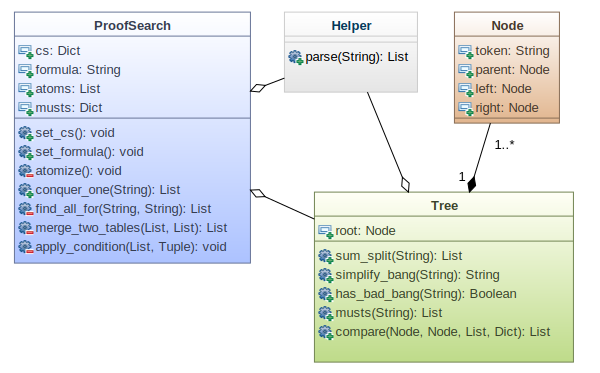
\includegraphics[scale=0.5]{uml.pdf}
\end{frame}

\subsubsection{Obstacles}
\begin{frame}
	Those were some of the problems that took the longest for me to figure out.
	\begin{itemize}
		\item[musts] How can a formula be broken down such that I know what I must be looking for in \emph{CS}.
		\item[compare] How to compare two trees and what to do with the result (\emph{Wilds!}).
		\item[Y-Wilds] What difference do they make when comparing \emph{musts} proof constants with \emph{CS} entries. Are all cases covered?
	\end{itemize}
\end{frame}

\subsection{Continuation}
\begin{frame}{What must still be done?}
\begin{itemize}
	\item Decide for a standard output. \\
	(Only True/False, table of must for which a configuration was found or all tables of musts for which a configuration was found.)
	\item A few in-code documentation additions.
	\item Final refactoring.
\end{itemize}
\end{frame}

\begin{frame}{What could be done?}
\begin{itemize}
	\item Add more logic operators. \\
	(such as $\vee, \wedge, ¬$)
	\item User-friendly GUI (simple) with input check.
	\item Clearly state assumptions and proof them.
\end{itemize}
\end{frame}

\subsection{Conclusion}
\begin{frame}{Personal Conclusion}
	\begin{center}
	\begin{itemize}
		\item new language
		\item riddling with logic
		\item implementing an algorithm
		\item clean coding (documentation and presentation)
	\end{itemize}
	\end{center}
\end{frame}

\begin{frame}{Question?}

\end{frame}
\end{document}

